\section{Etude Exp\'erimentale avec des diff\'erentes paramètres}
\newtheorem{theo}{th\'eor\`eme: }
\newtheorem{defe}{d\'efinition:}
\newtheorem{forule}{}

\noindent Pour nos expérimentations nous nous sommes concentrés sur les 3 modèles (avec des différents taux de service mais $\mu$=5 requêtes/h) suivant : \begin{itemize}
    \item modèle A (12 VMs de 1 coeur avec chacune un taux de service $\mu$) 
    \item modèle B (6 VMs de 2 coeur avec chacune un taux de service 2*$\mu$)
    \item modèle C (3 VMs de 4 coeur avec chacune un taux de service 4*$\mu$) \\
\end{itemize}


\noindent On a  également réalisé nos test avec différentes valeurs pour $\lambda$ : \begin{itemize}
    \item 50
    \item 60
    \item 70
    \item 80 
    \item 90
    \item 100\\
\end{itemize}

\noindent On définie que la capacité du système B est égal à 100.

\noindent Et enfin on l'a simulé sur la grande période à laquelle on l'effectue et attend son statut stable. Et après, on compare les résultats afin de déterminer la plus optimale.

\subsection{Résultats}
\subsubsection{Tableaux de performances}

\vspace{1cm}
\quad \\
\begin{tabular}{|c|c|c|c|c|}
\hline
\multicolumn{3}{|c}{modèle C : 3 MV} &\multicolumn{1}{c}{$\mu=20$}&\\
\hline 
\multicolumn{1}{|c|}{lambda}& \multicolumn{1}{c|}{resultat} & \multicolumn{1}{c|}{Pr blocage} & \multicolumn{1}{c|}{nbr requetes} & \multicolumn{1}{c|}{nbr MVs}  \\
\hline
 \multirow{2}{*}{$\lambda = 50$} & simulation & 0.0004011 & 61.7 & 2.236 \\ \cline{2-5}
                            & analytique & 0.0001695 & 65.97 & 2.4995 \\
                            \hline
  \multirow{2}{*}{$\lambda = 60$} & simulation & 0.01112 & 72.39 & 2.654 \\ \cline{2-5}
                            & analytique & 0.0263157 & 81.42056 & 2.92105 \\ \hline
  \multirow{2}{*}{$\lambda = 70$} & simulation & 0.1316 & 92.81 & 2.982 \\ \cline{2-5}
                            & analytique & 0.1432906 & 94.113288 & 2.998482 \\ \hline
  \multirow{2}{*}{$\lambda = 80$} & simulation & 0.2394 & 96.56 & 2.997 \\ \cline{2-5}
                            & analytique & 0.25 & 97.000784 & 2.999979 \\ \hline
  \multirow{2}{*}{$\lambda = 90$} & simulation & 0.3235 & 97.75 & 2.998 \\ \cline{2-5}
                            & analytique & 0.33333 & 98.00001 & 2.9999999 \\ \hline
  \multirow{2}{*}{$\lambda = 100$} & simulation & 0.3917 & 98.33 & 2.998 \\ \cline{2-5}
                            & analytique & 0.4 & 98.5 & 2.99999999 \\ \hline
\end{tabular}  

\vspace{1cm} \quad \\
\begin{tabular}{|c|c|c|c|c|}
\hline
\multicolumn{3}{|c}{modèle C : 6 MV} &\multicolumn{1}{c}{$\mu=10$}&\\
\hline 
\multicolumn{1}{|c|}{lambda}& \multicolumn{1}{c|}{resultat} & \multicolumn{1}{c|}{Pr blocage} & \multicolumn{1}{c|}{nbr requetes} & \multicolumn{1}{c|}{nbr MVs}  \\
\hline
 \multirow{2}{*}{$\lambda = 50$}  & simulation & 0 & 59.94 & 4.243 \\ \cline{2-5}
                            & analytique & 0.000841 & 71.6329 & 4.99579 \\ \hline
                            
  \multirow{2}{*}{$\lambda = 60$} & simulation & 0.002463 & 72.8 & 5.036 \\ \cline{2-5}
                            & analytique & 0.03726 & 86.634695 & 5.776433 \\ \hline
  \multirow{2}{*}{$\lambda = 70$}  & simulation & 0.09933 & 88.66 & 5.726 \\ \cline{2-5}
                            & analytique & 0.145723 & 94.491871 & 5.9799 \\ \hline
  \multirow{2}{*}{$\lambda = 80$}  & simulation & 0.2401 & 96.34 & 5.969 \\ \cline{2-5}
                            & analytique & 0.250198 & 97.018786 & 5.99841 \\ \hline
  \multirow{2}{*}{$\lambda = 90$}& simulation & 0.3307 & 97.82 & 5.99 \\ \cline{2-5}
                            & analytique & 0.33335 & 98.001165 & 5.999849 \\ \hline
  \multirow{2}{*}{$\lambda = 100$} & simulation & 0.3973 & 98.29 & 5.992 \\ \cline{2-5}
                            & analytique & 0.4 & 98.500101 & 5.99998 \\ \hline
\end{tabular}  
\vspace{1cm}  \quad \\
\begin{tabular}{|c|c|c|c|c|}
\hline
\multicolumn{3}{|c}{modèle C : 12 MV} &\multicolumn{1}{c}{$\mu=5$}&\\
\hline 
\multicolumn{1}{|c|}{lambda}& \multicolumn{1}{c|}{resultat} & \multicolumn{1}{c|}{Pr blocage} & \multicolumn{1}{c|}{nbr requetes} & \multicolumn{1}{c|}{nbr MVs}  \\
\hline
 \multirow{2}{*}{$\lambda = 50$}& simulation & 0 & 45 & 6.37 \\ \cline{2-5}
                            & analytique & 0.001881 & 75.48 & 9.98 \\ \hline
  \multirow{2}{*}{$\lambda = 60$}  & simulation & 0 & 53.4 & 7.457 \\ \cline{2-5}
                            & analytique & 0.0459 & 88.83 & 11.44 \\ \hline
  \multirow{2}{*}{$\lambda = 70$}  & simulation & 0 & 66.85 & 9.068 \\ \cline{2-5}
                            & analytique & 0.15 & 94.91 & 11.89 \\ \hline
  \multirow{2}{*}{$\lambda = 80$} & simulation & 0.0369 & 76.24 & 10.03 \\ \cline{2-5}
                            & analytique & 0.25 & 97.08 & 11.98 \\ \hline
  \multirow{2}{*}{$\lambda = 90$} & simulation & 0.2254 & 90.81 & 11.23 \\ \cline{2-5}
                            & analytique & 0.3335 & 98.011 & 11.995 \\ \hline
  \multirow{2}{*}{$\lambda = 100$} & simulation & 0.3562 & 96.09 & 11.72 \\ \cline{2-5}
                            & analytique & 0.40005 & 98.50 & 11.998 \\ \hline
\end{tabular}  

\begin{comment}
\subsubsection{Analyses}
On observe que globalement l'accélération est efficace pour une période allant de 10 à 20. En revanche il faut noter que l'effet est positif seulement lorsque $\alpha$ est proche de 1. Ainsi dans nos experimentations les améliorations se font surtout dans le cas où $\alpha$ = 0.95.
\\

En général on observe un gain qui va jusqu'à 14\% (cas du graphe de l'Inde avec une période de 10). En revanche il semble que certaines topologies se prêtent très mal à cet algorithme, par exemple plus la période est basse pour le graphe de Stanford et plus la convergence est lente. On observe même une absence de convergence quand la période est de 5. Globalement il semble qu'une période trop petite soit très risquée : il semble plus rentable d'augmenter la période d'accélération pour réduire le temps(sec) moyen de calcul.
\end{comment}
%\newpage

\subsection{Analyses de graphes}
\begin{figure}[ht!]
\centering
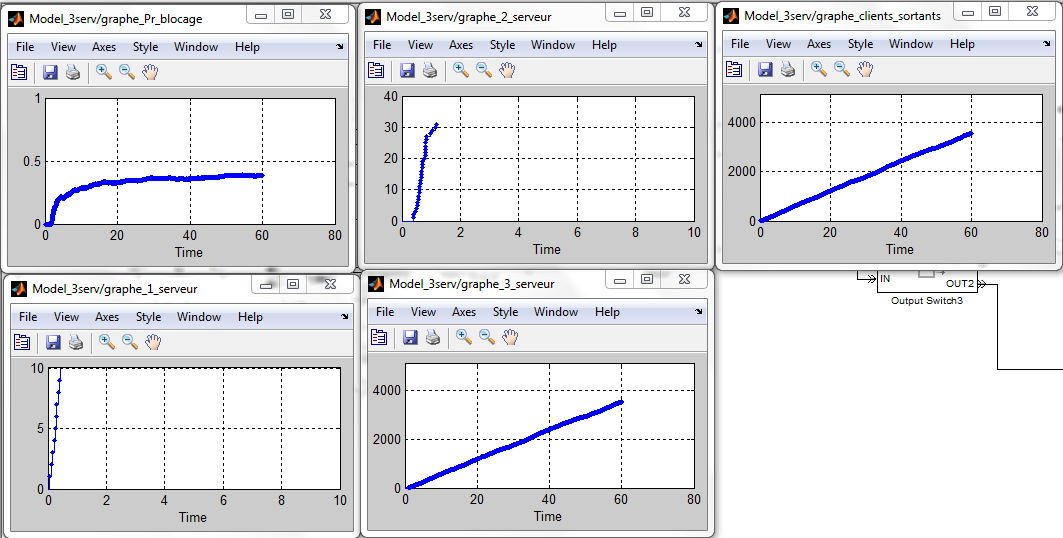
\includegraphics[width=0.95 \textwidth]{photo/graphe_model_3MV.png}
\caption{Les graphes de simulation avec 3 MVs et le paramètre $\lambda$=100}
\label{fig:graphe1}
\end{figure}
\newpage
\noindent Ces graphes représentent les résultats de la simulation du Modèle C avec les paramètres suivants: 3VM, Taux d’arrivées  $\lambda$=100, Taux de service  4$\mu$ ( $\mu$=5 requêtes/h) et la Capacité du système B=100.

Nous obtenons 5 graphes (graphe de: probabilité de blocage, les clients(ou taches) passé par un serveur, les clients passé par deux serveurs, les clients passés par trois serveurs et les client passé par le système) en prenant un temps réduit de la simulation (60) pour avoir des graphes lisibles.

"graphe$\_$Pr$\_$blocage" c'est le graphe de probabilité de blocage qui montre que dans les premiers temps un blocage nul cela indique que tous les clients arrivés sont bien servis. Dès que la courbe dépasse la valeur 0, tous les serveurs sont activé car on a utilisé la distribution exponentielle pour générer des clients (le taux d'arrivées augmente selon la loi exponentielle), on remarque une augmentation progressive de la probabilité de blocage par rapport au temps car le taux d'arrivées est toujours en augmentation. au temps supérieur à 20 la courbe devient presque stable.

"graphe$\_$1$\_$serveur"," graphe$\_$2$\_$serveur ", "graphe$\_$3$\_$serveur" sont des graphes représentant le nombre de clients servis par 1, 2 ou 3 serveurs par rapport au temps. "graphe$\_$1$\_$serveur" montre que dans les premiers temps les clients sont servis par un seul serveur.

"graphe$\_$2$\_$serveur " commence après que le "graphe$\_$1$\_$serveur" atteint son seuil et qu'il a traité certains clients.

"graphe$\_$3$\_$serveur" commence quand le "graphe$\_$2$\_$serveur " atteint son seuil et  il continu à augmenter jusqu'à la fin de la simulation.

"graphe$\_$client$\_$sortants" ce graphe montre que tous les clients sont servis par le système, on remarque qu'il a la même allure que le "graphe$\_$3$\_$serveur". cela indique que les clients servis par ce système sont presque tous traités par les 3 serveurs  avec une probabilité de blocage due à un Taux d’arrivées plus élevé par rapport à la capacité de système.
\\
\newpage
\begin{figure}[ht!]
\centering
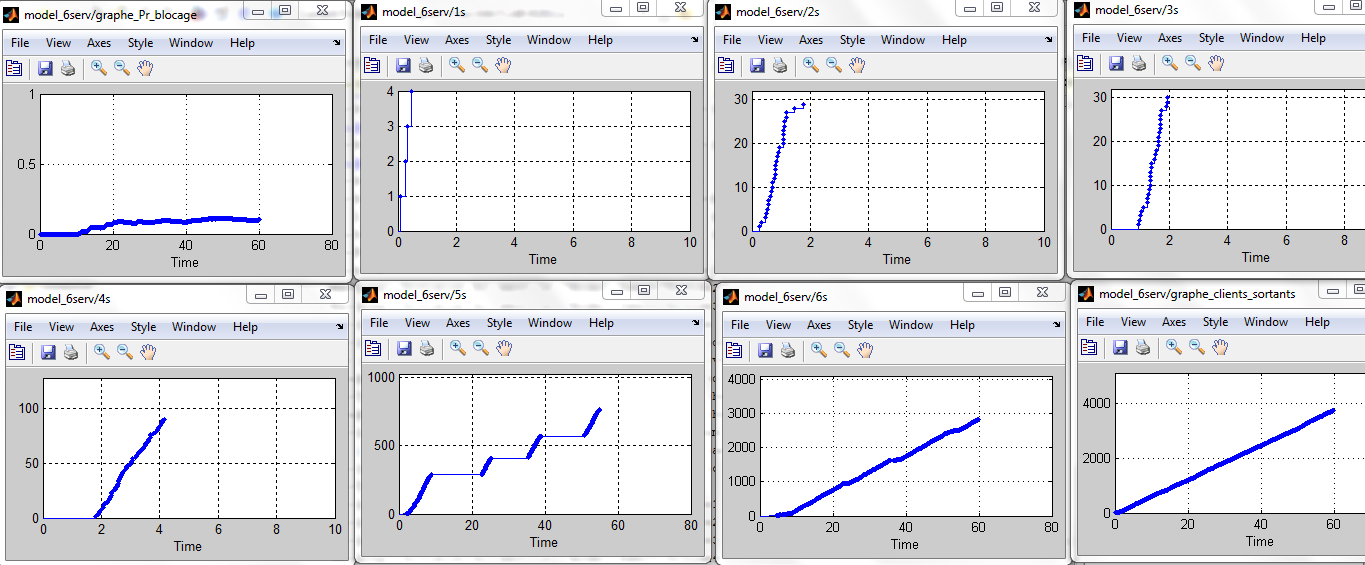
\includegraphics[width=0.95 \textwidth]{photo/graphe_6MV.png}
\caption{Les graphes de simulation avec 6 MVs et le paramètre $\lambda$=70}
\label{fig:graphe2}
\end{figure}
\noindent Ces graphes représentent les résultats de la simulation du Modèle B avec les paramètres suivants: 6VM, Taux d’arrivées  $\lambda$=70, Taux de service  2$\mu$($\mu$=5 requêtes/h) et la Capacité du système B=100.

\noindent Dans ce modèle on constate que le fonctionnement des serveur est similaire au fonctionnement des serveurs du modèle précédant (à chaque déplacement de seuil d'un serveur, le prochain  serveur se lance), le graphe "5s" montre que le les 5 serveurs fonctionnent de manière discontinue, cette discontinuité est due au déplacement de leur seuil ce qui entraine le fonctionnement avec 6 serveurs, lorsque le taux d'arrives est inferieur au seuil des 5 serveurs, le sixième serveur sera désactivé (fonctionnement en 5 serveurs).   

\noindent On observe que la probabilité de blocage a diminué par rapport au modèle précédant car on a simuler avec un taux d'arrivés  réduit
 \newpage
 \begin{figure}[ht!]
\centering
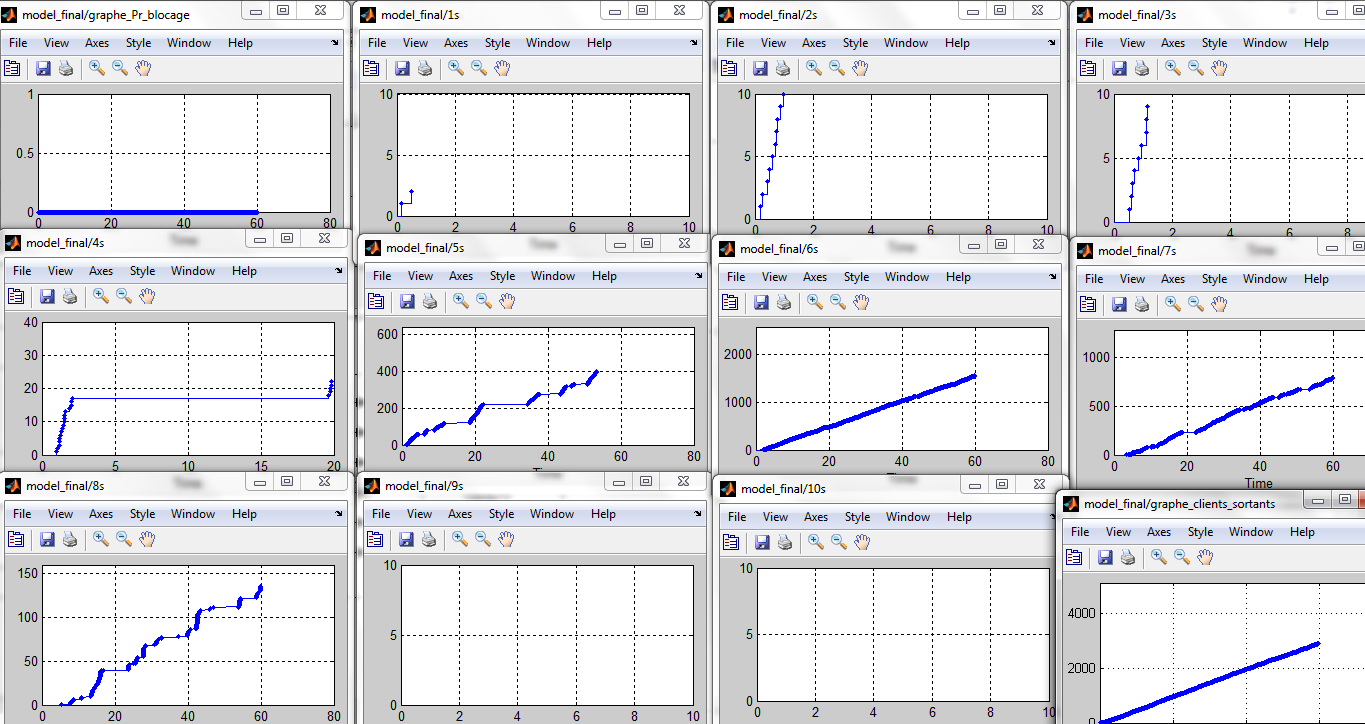
\includegraphics[width=0.95 \textwidth]{photo/graphe_12MV.png}
\caption{Les graphes de simulation avec 12 MVs et le paramètre $\lambda$=50}
\label{fig:graphe3}
\end{figure}
\noindent Ces graphes représentent les résultats de la simulation du Modèle A, avec les paramètres suivants: 12VM, Taux d’arrivées  $\lambda$=50, Taux de service  $\mu$=5 requêtes/h et la Capacité du système B=100.

Dans ce modèle on voie le même principe de fonctionnement des serveurs comme les modèles précédents. de plus, il n'existe aucune courbe sur les graphes "9s", "10s", "11s" et "12s" car le taux d'arrivées n'a pas dépasser le seuil de "8s" de ce fait, la probabilité de blocage est toujours nulle comme le montre le graphe"graphe$\_$Pr$\_$blocage".


 



